\section{Preliminaries}

The User Space component is a server process that provides the web service. Its main tasks are to mediate the services of the translation memory and to reflect all the users' GUI activity and make the user's work available always in the same state she finished her work.

The User Space is a Java Servlet which is run using the \emph{Jetty WebServer}. All of the User Space code is implemented Java. It uses \emph{Hibernate} object-relational mapping library. The same \emph{PostgreSQL} database as in the TM Core is used. The in-memory \emph{hsqldb} database is used for the unit testing.

Because the TM Core is a separate module it is also linked as dependency to the User Space.

\section{Architecture}

We try to use as most as possible from the shared classes and prevent using the User Space specific classes. If some additional functionality is required and cannot be incorporated into the shared classes, mostly the database and core calls, we wrap the shared classes into distinct User Space classes.

The server class which processes the calls on the first level contains the Session objects. These objects processes the calls with association the the particular logged in users. These two classes are not a part of the shared classes set.

The session class contains an object representing the user (a wrapper for the shared class). Hash tables of active documents and active chunks is there to access them faster than by searching lists in the user and document objects. Both the document objects and translation results objects which collect the source chunk, translation suggestion and the actual user's translation are wrappers for the shared classes. Anyway, the inner shared objects are used for communication with other components.

The more basic level than the translation result uses exactly the shared classes structure.

\section{Functionality overview}

Most of the functionality of the User Space is available via the RPC calls from the client side. During the run of the server there exist one instance of the server class. The main task of the sever class is to process the calls from the clients -- which in fact means pass the calls further to the particular sessions and manage the sessions. It has a method for every single operation that is possible to happen in the client.

After the user logs in, a Session object is created. It contains a unique session ID the client uses for authentication of its calls. A session object contains information about the user o -- the settings and a list of the documents owned by the user, and hash tables of documents and chunks which are currently in use. 

Until the user does not explicitly request a document, only basic information about the document remains loaded into memory (basic facts about the movie, time of last changes of the document). Only if he opens the document for editing, all the document chunks with the translation suggestions and already finished users translations are loaded.

There is also a thread running in the server that checks the time how long the sessions are opened without any users action. If this time exceeds the predefined session time out limit, the session is terminated. The other way of terminating a session is when the user logs out. In both of these cases the changes the user made which were stored just in the memory so far, are saved permanently to the database. It is also possible to close just a document, which will also lead to saving all the document content to the database immediately.

\begin{figure}
\begin{center}
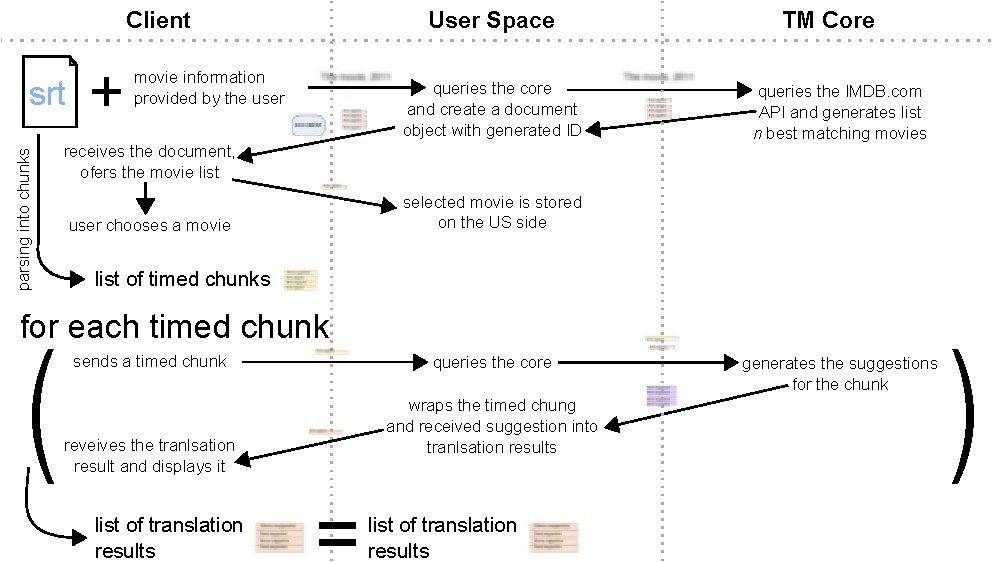
\includegraphics{figures/creating_document.pdf}
\end{center}
\caption{Structure of component communication during a new document creation}
\end{figure}

When a new document is created, the User Space receives a basic information about the movie first. Based on that it creates a Document object and saves it to the database immediately, to receive a unique  database ID which is the used as a document identifier in all other calls. The core is called at this moment to provide a list of possible movies with best matching title and year of production together with genre tags obtained from the IMDB.com. The user is then supposed to choose one or none of the suggested movies. This information is used by the User Space at the moment the core is queried for the translation suggestions.

When a new document is created, the client application starts to send the batches of chunks which are supposed to be translated. When the User Space receives such call, it queries the TM Core for the translation suggestion and adds the chunks to the list list chunks which the appropriate document consists of.

User Space also provides feedback to the core. A list of new translation the users produced can be generated together with information which translation suggestions were post-edited.

\section{Implementation Details}
\subsection{The Data Types Overview}

The User Space uses the shared data types used thorough the application or the wrapper of such classes. A brief overview of the used classes and their role in the User Space follows. (Prefix US means User Space.)

\begin{itemize}
\item {\tt FilmtitBackendServer}  -- The class is the Java Servlet whose public methods are invoked by the RPC calls. Its main task is to mediate the calls to concrete opened sessions and take care of users login. A thread checking if there some sessions without activity for a long time and termites the non-active sessions is run the server class.

\item {\tt Session} -- The class represents a running session. There is exactly one session object for one logged in user, it is actually the Session class which process the client calls. It contains hash tables of actively edited documents and the chunks they contain to access them faster via the calls. During the existence of a session object all the client side operations are stored just in the memory. All the content is saved to database when the session is terminated. The existence of sessions is saved to the database to provide some basic statistics about using the application.

\item {\tt USUser} -- This class is a wrapper of the shared User class. During the existence of the session its used as a provider of the documents owned by the user. It is also used for storing the settings of the user. In advance to the shared class a set of documents which has been left opened when the last user's session was terminated is also stored in the class which is used at the time a new session is created. 

\item {\tt USDocument} -- The class is a wrapper of the shared {\tt Document} class. A {\tt USDocument} object represents a subtitle file with additional information about the movie it belongs to. Its content is supposed to be a mirror image of the Document object on the client side. It contains a list of Translation Results representing the actual subtitle chunks if the document is loaded to be edited.

\item {\tt USTranslationResult} -- It is a wrapper for the shared {\tt TranlsationResult} class. The class congregates the original subtitle chunk, its timing, the translation suggested by translation memory and the result of the user activity -- the user's translation which translation suggestion she has chosen. It is the class where the actual translation is being done. Despite a user can delete the document he is working all the translation results are kept in the database to provide a  feed back to the translation memory.

\item {\tt TimedChunk} -- It is a shared class which is used for the communication with the client. When the User Space receives a Timed Chunk it wraps it into a Tranlsation Result and send it back to the client together with the translation memory suggestion.

\item {\tt TranslationPair} -- A list {\tt TranslationPair} objects is received as a respond from the Translation Memory Core. It is then stored in the Translation Results objects both on the server and client side.
\end{itemize}

\subsection{Database Mapping}

As was mentioned many times before, the User Space mirrors all the client operations and make them persistent on the server side. The persistence ensured by saving the data to the database. The exist many sophisticated tool for Java to ensure the data persistence, e.g. \emph{Java Persistence API} framework which or some frameworks working on the higher level of abstraction as \emph{Spring Data Framework}. Since only very basic database operations are required during the run of the User Space -- loading and saving of the raw Java object -- only a object relational mapping is library used, concretely \emph{Hibernate}, in contrast to the core which uses just the JDBC connection.

Usually the mapping just reflects the data properties of a classes. If the class is a wrapper of a shared class the getters and setters of the properties are bind to the wrapped objects properties.

The mapping of {\tt USDocument} does not include the list of Translation Results the document contains. The reason is that potentially a lot documents can be loaded because they are owned by a user, but only a few of them, most probably just one will be really edited during a session and it will be necessary to load all of the Translation Results with the suggestions to the memory. It would be also possible to use the lazy Hibernate collection mapping, but it would require to have an opened database session during the first access to the collection. Instead of theis the Translation Results are loaded from the database explicitly in a separate method which should contribute to the readability of the code.

The only non-trivial case of the mapping is the {\tt USUser} class which contains set of documents which were active at the time when the last user session was terminated and the list of documents the user owns. This is solved by the Hibernate one-to-many mapping which takes control over loading the whole object structure at once. There are just the foreign keys in the database, whereas the collection of complete objects are loaded.


